\section{Die Raupe Nummersatt und die probabilistische Methode}
Eine besonders schwere Aufgabe wurde bei der Bundesrunde 2003 gestellt:

\begin{aufgabe*}[***]\label{aufgabe:RaupeNummersatt}
	Gegeben ist ein Quadratgitter aus $N \times N$ Kästchen; $N\geqslant 3$ sei eine ungerade Zahl.
	Die Raupe Nummersatt sitzt in dem Kästchen genau in der Mitte des Gitters. Jedes der übrigen
	Kästchen enthält eine positive ganze Zahl. Über die Verteilung der Zahlen ist nur bekannt, dass
	sich in keinen zwei Feldern die gleiche Zahl befindet.
	Nummersatt möchte durch dieses Zahlenmeer einen Weg nach draußen finden. Sie kann dabei
	von einem Kästchen stets nur zu einem entlang einer Seite angrenzenden Kästchen weiterwandern
	und muss jede Zahl fressen, durch deren Kästchen ihr Weg führt. Jede Zahl $n$ wiegt $\frac{1}{n}\operatorname{kg}$, und
	Nummersatt kann insgesamt nicht mehr als $2\operatorname{kg}$ Zahlen fressen.
	Untersuche
	\begin{enumerate}[label={$(\alph*)$},ref={$(\alph*)$}]
		\item für $N = 2003$,
		\item für alle ungeraden Zahlen $N\geqslant 3$,
	\end{enumerate}
	ob die Zahlen im Gitter so ungünstig verteilt sein können, dass Nummersatt keinen Weg nach
	draußen finden kann, auf dem höchstens $2\operatorname{kg}$ Zahlen liegen.
\end{aufgabe*}

In diesem Kapitel wollen wir eine Lösung dieser Aufgabe vorstellen. Wir werden zeigen, dass die Raupe Nummersatt in beiden Aufgabenteilen stets einen Weg nach draußen findet und dass die geforderten maximal $2\operatorname{kg}$ sogar durch $1\operatorname{kg}$ ersetzt werden können.

\subsection*{Die probabilistische Methode}

Der Lösung, die wir präsentieren werden, liegt eine der wichtigsten Methoden in der Kombinatorik zugrunde: Die \emph{probabilistische Methode:}
\begin{enumerate}\itshape
	\item[$(*)$] Wenn es sich als schwierig erweist, ein Objekt mit einer gewünschten Eigenschaft~$E$ direkt zu konstruieren, dann versuche stattdessen zu zeigen, dass ein \enquote{zufällig ausgewähltes Objekt} die Eigenschaft~$E$ \enquote{im Erwartungswert} erfüllt.
\end{enumerate}
Natürlich kann das nicht immer klappen. Die probabilistische Methode lohnt sich nur dann, wenn wir ohnehin vermuten, dass die Eigenschaft~$E$ in Wirklichkeit gar nicht so selten vorkommt. Aber wenn die Methode funktioniert, führt sie oftmals zu außerordentlich eleganten Lösungen. Auch in der modernen mathematischen Forschung findet die probabilistische Methode vielfach Anwendung und es gibt viele phantastische Resultate, die sich nur auf diese Weise beweisen lassen.

Wir werden nun die probabilistische Methode anhand von Aufgabe~\ref{aufgabe:RaupeNummersatt} demonstrieren. Die Lösung ist so formuliert, dass nachvollziehbar ist, wie wir darauf gekommen sind. In der Olympiade würdet ihr diese Überlegungen natürlich weglassen und nur die relevanten Begründungen aufschreiben.

\begin{proof}[Lösung zu Aufgabe~\ref{aufgabe:RaupeNummersatt}]
	Wir beginnen mit einigen Bezeichnungen. Wenn $W$ ein Weg ist, dann identifizieren wir $W$ mit der Menge seiner Felder, sodass $f\in W$ bedeutet, dass $f$ ein Feld von $W$ ist. Wenn~$f$ ein Feld ist, dann bezeichnen wir mit $n(f)$ die natürliche Zahl, die auf~$f$ steht. Unser Ziel ist, eine geeignete Menge $\mathcal W$ von nach draußen führenden Wegen sowie nichtnegative Gewichte $p(W)\geqslant 0$ für $W\in\mathcal W$ zu finden, sodass $\sum_{W\in \mathcal W}p(W)=1$ gilt und außerdem die folgende Ungleichung erfüllt ist:
	\begin{equation*}
		\sum_{W\in \mathcal{W}} p(W)\sum_{f\in W} \frac{1}{n(f)}<1\,.
	\end{equation*}
	Dann muss es nämlich einen Weg $W\in\mathcal W$ geben, sodass das Gewicht der Zahlen auf $W$ kleiner als $1$ ist. Wir können $p(W)$ als die \enquote{Wahrscheinlichkeit, dass $W$ ausgewählt wird} interpretieren und die obige Summe dann als den Erwartungswert des Gewichtes der Zahlen auf $W$.
	
	Bevor wir uns an den Beweis dieser Ungleichung machen können, müssen wir zwei entscheidende Fragen beantworten:
	\begin{enumerate}[label={$(\arabic*)$},ref={$(\arabic*)$}]\itshape
		\item Was ist eine geeignete Wahl für die Menge $\mathcal W$?\label{frage:WasIstW?}
		\item Was ist eine geeignete Wahl für die Gewichte $p(W)$, $W\in\mathcal W$?\label{frage:WasFuerGewichte?}
	\end{enumerate}
	Eine \enquote{geeignete Wahl} ist eine Wahl, für die die gewünschte Ungleichung nicht nur erfüllt ist, sondern sich auch möglichst einfach beweisen lässt. Unsere Erfahrung mit Olympiade-Aufgaben sagt uns, dass ein Beweis der gewünschten Ungleichung vermutlich mit folgender Umsortierung der fraglichen Summe beginnen würde:
	\begin{equation*}
		\sum_{W\in \mathcal{W}} p(W)\sum_{f\in W} \frac{1}{n(f)}=\sum_{f\in\mathcal F}\frac{1}{n(f)}\sum_{W\in \mathcal W_f}p(W)\,.
	\end{equation*}
	Hierbei bezeichnet $\mathcal F$ die Menge aller Felder, die die Wege aus $\mathcal W$ durchlaufen, und für $f\in \mathcal F$ ist $\mathcal W_f\subseteq \mathcal W$ die Teilmenge $\braces*{W\in\mathcal W\ \middle|\ f\in W}$. Für die innere Summe auf der rechten Seite schreiben wir kurz $p(f)$, also\footnote{Wenn $p(W)$ in der stochastischen Interpretation die Wahrscheinlichkeit angibt, mit der der Weg $W$ gewählt wurde, dann ist $p(f)$ die Wahrscheinlichkeit dafür, dass der gewählte Weg das Feld~$f$ enthält. Die obige Umsortierung der Summe lässt sich in der stochastischen Interpretation mithilfe von charakteristischen Funktionen und der Linearität des Erwartungswertes herleiten. Das ist aber deutlich umständlicher, als einfach die Summe umzusortieren.}
	\begin{equation*}
		p(f)\coloneqq\sum_{W\in\mathcal{W}_f}p(W)\,.
	\end{equation*}
	Unser Problem würde sich sicherlich deutlich vereinfachen, wenn wir eine einfache Beschreibung für $p(f)$ hätten. Wie einfach? Können wir erreichen, dass alle $p(f)$ gleich sind? Definitiv nicht. Denn je weiter $f$ vom Ursprung ist, desto weniger Wege führen durch $f$. Die nächstbeste Hoffnung wäre dann, dass $p(f)$ nur vom Abstand zwischen dem Ursprung und~$f$ abhängt. Der \enquote{Abstand} bezeichnet hier natürlich nicht den euklidischen Abstand, sondern die Anzahl der Felder auf einem minimalen Weg vom Ursprung nach~$f$.
	
	Für jedes $\ell\geqslant 0$ betrachten wir also die Menge $\mathcal R_\ell$ aller Felder, die vom Ursprung den Abstand $\ell$ haben. Ferner sei $\mathcal F_\ell=\bigcup_{k\leqslant \ell}\mathcal R_k$; dann ist $\mathcal F_\ell$ die Menge aller Felder, die sich vom Ursprung aus in maximal $\ell$ Schritten erreichen lassen. \enquote{Aus der Ferne betrachtet} sieht $\mathcal F_\ell$ aus wie ein auf der Ecke balanciertes Quadrat und $\mathcal R_\ell$ sieht aus wie dessen Rand. Wenn wir die Mittelpunkte der Kästchen in $\mathcal R_\ell$ verbinden, erhalten wir sogar ein tatsächliches Quadrat $\mathcal Q_\ell$.
	
	\begin{figure}[ht]
		\centering
		\begin{tabularx}{\textwidth}{X c X c X c X}
			& \begin{tikzpicture}[x=0.28cm,y=0.28cm]
				\draw (-7.5,-0.5)%
				% linke Ecke
				to ++(0,1) to ++ (1,0) to ++(0,1) to ++(1,0) to ++(0,1) to ++ (1,0) to ++(0,1) to ++ (1,0) to ++(0,1) to ++ (1,0) to ++(0,1) to ++ (1,0) to ++(0,1) to ++ (1,0) to ++(0,1) to ++ (1,0)%
				% obere Ecke
				to ++(0,-1) to ++(1,0) to ++(0,-1) to ++(1,0) to ++(0,-1) to ++(1,0) to ++(0,-1) to ++(1,0) to ++(0,-1) to ++(1,0) to ++(0,-1) to ++(1,0) to ++(0,-1) to ++(1,0) to ++(0,-1)%
				% rechte Ecke		
				to ++(-1,0) to ++(0,-1) to ++(-1,0) to ++(0,-1) to ++(-1,0) to ++(0,-1) to ++(-1,0) to ++(0,-1) to ++(-1,0) to ++(0,-1) to ++(-1,0) to ++(0,-1) to ++(-1,0) to ++(0,-1) to ++(-1,0)%
				% untere Ecke 
				to ++(0,1) to ++(-1,0) to ++(0,1) to ++(-1,0) to ++(0,1) to ++(-1,0) to ++(0,1) to ++(-1,0) to ++(0,1) to ++(-1,0) to ++(0,1) to ++(-1,0) to ++(0,1) to cycle;
				\draw (-6.5,-0.5) to ++(0,1) to ++ (1,0) to ++(0,1) to ++(1,0) to ++(0,1) to ++ (1,0) to ++(0,1) to ++ (1,0) to ++(0,1) to ++ (1,0) to ++(0,1) to ++ (1,0) to ++(0,1) to ++ (1,0) %
				% obere Ecke
				to ++(0,-1) to ++(1,0) to ++(0,-1) to ++(1,0) to ++(0,-1) to ++(1,0) to ++(0,-1) to ++(1,0) to ++(0,-1) to ++(1,0) to ++(0,-1) to ++(1,0) to ++(0,-1)%
				% rechte Ecke		
				to ++(-1,0) to ++(0,-1) to ++(-1,0) to ++(0,-1) to ++(-1,0) to ++(0,-1) to ++(-1,0) to ++(0,-1) to ++(-1,0) to ++(0,-1) to ++(-1,0) to ++(0,-1) to ++(-1,0)%
				% untere Ecke 
				to ++(0,1) to ++(-1,0) to ++(0,1) to ++(-1,0) to ++(0,1) to ++(-1,0) to ++(0,1) to ++(-1,0) to ++(0,1) to ++(-1,0) to ++(0,1) to cycle;
				%\draw [line width=0.3,dash pattern=on 0.07cm off 0.07cm,dash phase=0.035cm] (-0.5,-0.5) to ++(0,1) to ++(1,0) to ++(0,-1) to cycle;
				%\draw[fill=black] (0,0) circle (2pt) node[shift={(-65:2.5ex)}] {$O$};
			\end{tikzpicture} & & 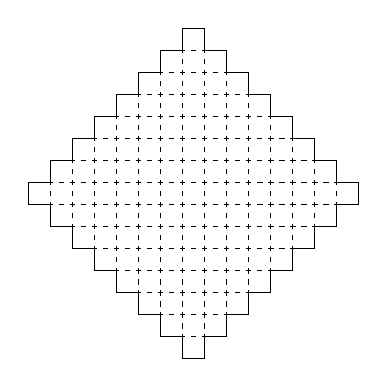
\begin{tikzpicture}[x=0.28cm,y=0.28cm]
				\draw (-7.5,-0.5)%
				% linke Ecke
				to ++(0,1) to ++ (1,0) to ++(0,1) to ++(1,0) to ++(0,1) to ++ (1,0) to ++(0,1) to ++ (1,0) to ++(0,1) to ++ (1,0) to ++(0,1) to ++ (1,0) to ++(0,1) to ++ (1,0) to ++(0,1) to ++ (1,0)%
				% obere Ecke
				to ++(0,-1) to ++(1,0) to ++(0,-1) to ++(1,0) to ++(0,-1) to ++(1,0) to ++(0,-1) to ++(1,0) to ++(0,-1) to ++(1,0) to ++(0,-1) to ++(1,0) to ++(0,-1) to ++(1,0) to ++(0,-1)%
				% rechte Ecke		
				to ++(-1,0) to ++(0,-1) to ++(-1,0) to ++(0,-1) to ++(-1,0) to ++(0,-1) to ++(-1,0) to ++(0,-1) to ++(-1,0) to ++(0,-1) to ++(-1,0) to ++(0,-1) to ++(-1,0) to ++(0,-1) to ++(-1,0)%
				% untere Ecke 
				to ++(0,1) to ++(-1,0) to ++(0,1) to ++(-1,0) to ++(0,1) to ++(-1,0) to ++(0,1) to ++(-1,0) to ++(0,1) to ++(-1,0) to ++(0,1) to ++(-1,0) to ++(0,1) to cycle;
				\begin{scope}[line width=0.3,dash pattern=on 0.07cm off 0.07cm,dash phase=0.035cm]
					\draw (-0.5,6.5) to (0.5,6.5);
					\draw (-1.5,5.5) to (1.5,5.5);
					\draw (-2.5,4.5) to (2.5,4.5);
					\draw (-3.5,3.5) to (3.5,3.5);
					\draw (-4.5,2.5) to (4.5,2.5);
					\draw (-5.5,1.5) to (5.5,1.5);
					\draw (-6.5,0.5) to (6.5,0.5);
					\draw (-0.5,-6.5) to (0.5,-6.5);
					\draw (-1.5,-5.5) to (1.5,-5.5);
					\draw (-2.5,-4.5) to (2.5,-4.5);
					\draw (-3.5,-3.5) to (3.5,-3.5);
					\draw (-4.5,-2.5) to (4.5,-2.5);
					\draw (-5.5,-1.5) to (5.5,-1.5);
					\draw (-6.5,-0.5) to (6.5,-0.5);
					\draw (6.5,-0.5) to (6.5,0.5);
					\draw (5.5,-1.5) to (5.5,1.5);
					\draw (4.5,-2.5) to (4.5,2.5);
					\draw (3.5,-3.5) to (3.5,3.5);
					\draw (2.5,-4.5) to (2.5,4.5);
					\draw (1.5,-5.5) to (1.5,5.5);
					\draw (0.5,-6.5) to (0.5,6.5);
					\draw (-6.5,-0.5) to (-6.5,0.5);
					\draw (-5.5,-1.5) to (-5.5,1.5);
					\draw (-4.5,-2.5) to (-4.5,2.5);
					\draw (-3.5,-3.5) to (-3.5,3.5);
					\draw (-2.5,-4.5) to (-2.5,4.5);
					\draw (-1.5,-5.5) to (-1.5,5.5);
					\draw (-0.5,-6.5) to (-0.5,6.5);
				\end{scope}
			\end{tikzpicture} & & 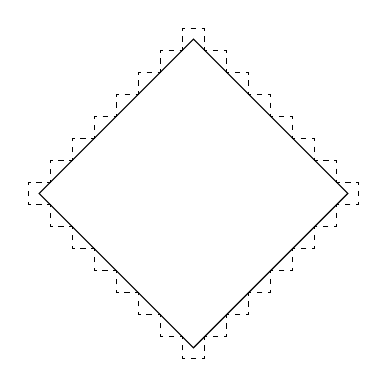
\begin{tikzpicture}[x=0.28cm,y=0.28cm]
				\draw [line width=0.3,dash pattern=on 0.07cm off 0.07cm,dash phase=0.035cm] (-7.5,-0.5)%
				% linke Ecke
				to ++(0,1) to ++ (1,0) to ++(0,1) to ++(1,0) to ++(0,1) to ++ (1,0) to ++(0,1) to ++ (1,0) to ++(0,1) to ++ (1,0) to ++(0,1) to ++ (1,0) to ++(0,1) to ++ (1,0) to ++(0,1) to ++ (1,0)%
				% obere Ecke
				to ++(0,-1) to ++(1,0) to ++(0,-1) to ++(1,0) to ++(0,-1) to ++(1,0) to ++(0,-1) to ++(1,0) to ++(0,-1) to ++(1,0) to ++(0,-1) to ++(1,0) to ++(0,-1) to ++(1,0) to ++(0,-1)%
				% rechte Ecke		
				to ++(-1,0) to ++(0,-1) to ++(-1,0) to ++(0,-1) to ++(-1,0) to ++(0,-1) to ++(-1,0) to ++(0,-1) to ++(-1,0) to ++(0,-1) to ++(-1,0) to ++(0,-1) to ++(-1,0) to ++(0,-1) to ++(-1,0)%
				% untere Ecke 
				to ++(0,1) to ++(-1,0) to ++(0,1) to ++(-1,0) to ++(0,1) to ++(-1,0) to ++(0,1) to ++(-1,0) to ++(0,1) to ++(-1,0) to ++(0,1) to ++(-1,0) to ++(0,1) to cycle;
				\draw (-7,0) to (0,7) to (7,0) to (0,-7) to cycle;
				%\draw [line width=0.3,dash pattern=on 0.07cm off 0.07cm,dash phase=0.035cm] (-0.5,-0.5) to ++(0,1) to ++(1,0) to ++(0,-1) to cycle;
				%\draw[fill=black] (0,0) circle (2pt) node[shift={(-65:2.5ex)}] {$O$};
			\end{tikzpicture} & \\\addlinespace
			& die Menge $\mathcal R_\ell$ & & die Menge $\mathcal F_\ell$ & & das Quadrat $\mathcal Q_\ell$ & 
		\end{tabularx}
	\end{figure}
	
	Es genügt zu zeigen, dass sich die Raupe Nummersatt stets aus der Menge $\mathcal F_\ell$ herausfressen kann, denn für $\ell\geqslant N$ kann das ursprüngliche $N\times N$-Quadrat in $\mathcal F_\ell$ platziert werden. Gleichzeitig haben wir damit auch nichts verschenkt, denn wir wollen ja die Aussage für beliebiges $N$ zeigen und $\mathcal F_\ell$ kann in einem $(2\ell+1)\times (2\ell+1)$-Quadrat platziert werden.
	
	Wir müssen immer noch eine geeignete Menge $\mathcal W$ von Wegen sowie geeignete Gewichte $p(W)$ bestimmen. Es liegt nahe, nur \enquote{direkte} Wege aus $\mathcal F_\ell$ heraus zu betrachten, weil alle anderen Wege nur unnötig Gewicht verschwenden. Was ist aber ein \enquote{direkter} Weg? Hier benutzen wir eine sehr elegante Idee: Für einen beliebigen Punkt $X$ auf dem Rand des Quadrats $\mathcal Q_\ell$ betrachten wir die Strecke $\overline{OX}$, wobei $O$ der Mittelpunkt des Ursprungskästchens ist. Sei $W(X)$ die Menge aller Kästchen, durch die $\overline{OX}$ verläuft. Dann ist $W(X)$ ein direkter Weg nach draußen! Hierbei müssen wir allerdings ein wenig aufpassen: Es kann nämlich passieren, dass $\overline{OX}$ durch einen Eckpunkt von Kästchen in $\mathcal F_\ell$ verläuft. In diesem Fall ist nicht so klar, welche der vier angrenzenden Kästchen zu $W(X)$ zählen sollen. Dieses Problem lösen wir, indem wir einfach nur diejenigen $X$ betrachten, für die $\overline{OX}$ durch keinen Eckpunkt von Kästchen verläuft. Damit schließen wir lediglich endlich viele Möglichkeiten für $X$ aus (nämlich für jeden Eckpunkt $E$ die Zentralprojektion von $E$ auf den Rand von $\mathcal Q_\ell$, also den Schnittpunkt des Strahls $\overrightarrow{OE}$ mit dem Rand von $\mathcal Q_\ell$).
	
	\begin{figure}[ht]
		\centering
		\begin{tabularx}{\textwidth}{X c X c X}
			& 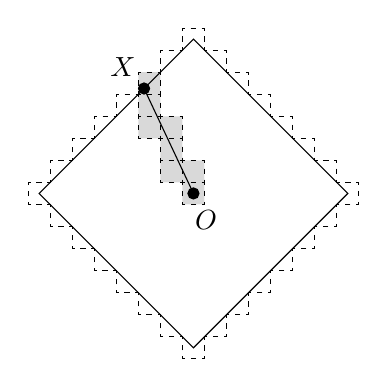
\begin{tikzpicture}[x=0.28cm,y=0.28cm]
				\begin{scope}[line width=0.3,dash pattern=on 0.07cm off 0.07cm,dash phase=0.035cm]
					\draw (-7.5,-0.5)%
					% linke Ecke
					to ++(0,1) to ++ (1,0) to ++(0,1) to ++(1,0) to ++(0,1) to ++ (1,0) to ++(0,1) to ++ (1,0) to ++(0,1) to ++ (1,0) to ++(0,1) to ++ (1,0) to ++(0,1) to ++ (1,0) to ++(0,1) to ++ (1,0)%
					% obere Ecke
					to ++(0,-1) to ++(1,0) to ++(0,-1) to ++(1,0) to ++(0,-1) to ++(1,0) to ++(0,-1) to ++(1,0) to ++(0,-1) to ++(1,0) to ++(0,-1) to ++(1,0) to ++(0,-1) to ++(1,0) to ++(0,-1)%
					% rechte Ecke		
					to ++(-1,0) to ++(0,-1) to ++(-1,0) to ++(0,-1) to ++(-1,0) to ++(0,-1) to ++(-1,0) to ++(0,-1) to ++(-1,0) to ++(0,-1) to ++(-1,0) to ++(0,-1) to ++(-1,0) to ++(0,-1) to ++(-1,0)%
					% untere Ecke 
					to ++(0,1) to ++(-1,0) to ++(0,1) to ++(-1,0) to ++(0,1) to ++(-1,0) to ++(0,1) to ++(-1,0) to ++(0,1) to ++(-1,0) to ++(0,1) to ++(-1,0) to ++(0,1) to cycle;
					\draw[fill=black!15!white] (-0.5,-0.5) to ++(0,1) to ++(-1,0) to ++(0,2) to ++(-1,0) to ++(0,3) to ++(1,0) to ++(0,-2) to ++(1,0) to ++(0,-2) to ++(1,0) to ++(0,-2) to cycle;
					\draw (-2.5,4.5) to (-1.5,4.5);
					\draw (-2.5,3.5) to (-1.5,3.5) to (-1.5,2.5) to (-0.5,2.5);
					\draw (-1.5,1.5) to (-0.5,1.5) to (-0.5,0.5) to (0.5,0.5);
				\end{scope}
				\draw (-7,0) to (0,7) to (7,0) to (0,-7) to cycle;
				\coordinate (X) at (0.32*-7,0.68*7);
				\draw (0,0) to (X);
				\draw[fill=black] (0,0) circle (2pt) node[shift={(-65:2.5ex)}] {$O$};
				\draw[fill=black] (X) circle (2pt) node[shift={(135:2.5ex)}] {$X$};
			\end{tikzpicture} & & 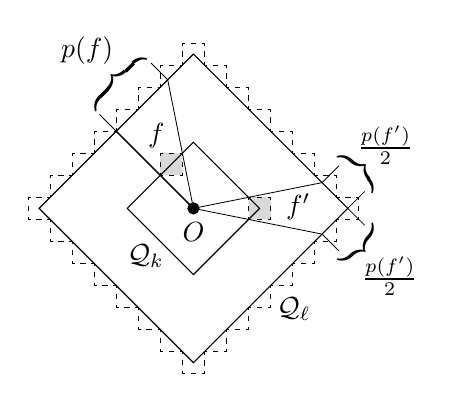
\begin{tikzpicture}[x=0.28cm,y=0.28cm]
				\begin{scope}[line width=0.3,dash pattern=on 0.07cm off 0.07cm,dash phase=0.035cm]
					\draw (-7.5,-0.5)%
					% linke Ecke
					to ++(0,1) to ++ (1,0) to ++(0,1) to ++(1,0) to ++(0,1) to ++ (1,0) to ++(0,1) to ++ (1,0) to ++(0,1) to ++ (1,0) to ++(0,1) to ++ (1,0) to ++(0,1) to ++ (1,0) to ++(0,1) to ++ (1,0)%
					% obere Ecke
					to ++(0,-1) to ++(1,0) to ++(0,-1) to ++(1,0) to ++(0,-1) to ++(1,0) to ++(0,-1) to ++(1,0) to ++(0,-1) to ++(1,0) to ++(0,-1) to ++(1,0) to ++(0,-1) to ++(1,0) to ++(0,-1)%
					% rechte Ecke		
					to ++(-1,0) to ++(0,-1) to ++(-1,0) to ++(0,-1) to ++(-1,0) to ++(0,-1) to ++(-1,0) to ++(0,-1) to ++(-1,0) to ++(0,-1) to ++(-1,0) to ++(0,-1) to ++(-1,0) to ++(0,-1) to ++(-1,0)%
					% untere Ecke 
					to ++(0,1) to ++(-1,0) to ++(0,1) to ++(-1,0) to ++(0,1) to ++(-1,0) to ++(0,1) to ++(-1,0) to ++(0,1) to ++(-1,0) to ++(0,1) to ++(-1,0) to ++(0,1) to cycle;
					%\draw (-0.5,2.5)  to ++(0,1) to ++ (1,0) %
					% obere Ecke
					%to ++(0,-1) to ++(1,0) to ++(0,-1) to ++(1,0) to ++(0,-1);
					%\draw (2.5,-0.5) %
					% rechte Ecke		
					%to ++(0,-1) to ++(-1,0) to ++(0,-1) to ++(-1,0) to ++(0,-1) to ++(-1,0)%
					% untere Ecke 
					%to ++(0,1) to ++(-1,0) to ++(0,1) to ++(-1,0) to ++(0,1) to ++(-1,0) to ++(0,1)%
					% linke Ecke
					%to ++ (1,0) to ++(0,1) to ++(1,0);
					\draw [fill=black!15!white] (-1.5,1.5) to ++(0,1) to ++(1,0) to ++(0,-1) to cycle;
					\draw [fill=black!15!white] (2.5,-0.5) to ++(0,1) to ++(1,0) to ++(0,-1) to cycle;
				\end{scope}
				\draw (-7,0) to (0,7) to (7,0) to (0,-7) to cycle;
				\draw (-3,0) to (0,3) to (3,0) to (0,-3) to cycle;
				\draw[fill=black] (0,0) circle (2pt) node[shift={(270:2ex)}] {$O$};
				\node[shift={(225:1.75ex)}] at (-1.5,-1.5) {$\mathcal Q_k$};
				\node[shift={(-45:2.75ex)}] at (3.5,-3.5) {$\mathcal Q_\ell$};
				\node[shift={(117:3.7)}] at (0,0) {$f$};
				\path (-3.5,3.5) to node[sloped,shift={(90:3ex)}] {$\overbrace{\hspace{0.924cm}}$} node[shift={(135:6.5ex)}] {$p(f)$} (-1.167,5.833);
				\draw[line width=0.3] (-3.5,3.5) to ++(135:2ex);
				\draw[line width=0.3] (-1.167,5.833) to ++(135:2ex);
				%\coordinate[shift={(45:2.75ex)}] (dummy) at (6.417,0.583);
				%\node [rotate=225] at (dummy) {$\boldsymbol{\big\lbrace}$};
				\path (5.833,1.167) to node[sloped,shift={(90:3ex)}] {$\overbrace{\hspace{0cm}}$} node[shift={(45:6ex)}] {$\frac{p(f')}{2}$} (7,0);
				\draw[line width=0.3] (5.833,1.167) to ++(45:2ex);
				\draw[line width=0.3] (7,0) to ++(45:2ex);
				\path (5.833,-1.167) to node[rotate=180,sloped,shift={(90:3ex)}] {$\overbrace{\hspace{0cm}}$} node[shift={(-45:6.5ex)}] {$\frac{p(f')}{2}$} (7,0);
				\draw[line width=0.3] (5.833,-1.167) to ++(-45:2ex);
				\draw[line width=0.3] (7,0) to ++(-45:2ex);
				\node[shift={(1:4.75)}] at (0,0) {$f'$};
				\draw [line width=0.3] (0,0) to (-3.5,3.5);
				\draw [line width=0.3] (0,0) to (-3.5,3.5);
				\draw [line width=0.3] (0,0) to (-3.5,3.5);
				\draw [line width=0.3] (0,0) to (-3.5,3.5);
				\draw [line width=0.3] (0,0) to (-1.167,5.833);
				\draw [line width=0.3] (0,0) to (5.833,1.167);
				\draw [line width=0.3] (0,0) to (5.833,-1.167);
			\end{tikzpicture} & \\\addlinespace
			& der Weg $W(X)$ & & geometrische Beschreibung von $p(f)$ & 
		\end{tabularx}
	\end{figure}
	
	Natürlich kann es Punkte $X\neq Y$ geben, für die $W(X)=W(Y)$ gilt. Wir können sogar genau sagen, wann das passiert: Die \enquote{verbotenen} Punkte, also die Zentralprojektionen der Ecken der Kästchen, teilen den Rand von $\mathcal Q_\ell$ in endlich viele Teilstrecken (bzw.\ Teilstrecken\emph{züge}: Die Ecken von $\mathcal Q_\ell$ sind \enquote{erlaubte Punkte}, also erhalten wir an den Ecken keine Strecken, sondern Streckenzüge mit einem Knick). Nun gilt $W(X)=W(Y)$ genau dann, wenn $X$ und $Y$ im Inneren der gleichen Teilstrecke (bzw.\ des gleichen Teilstreckenzuges) liegen. Ist $S$ eine solche Teilstrecke (bzw.\ ein solcher Teilstreckenzug), können wir
	also mit $W(S)$ den Weg bezeichnen, der sich für jedes $X\in S$ als $W(X)$ ergibt. Damit haben wir nun endlich einen Kandidaten für $\mathcal W$ gefunden: Wir wählen $\mathcal W$ als die Menge aller solcher $W(S)$. Gleichzeitig gibt es einen offensichtlichen Kandidaten für die Gewichte $p(W)$, $W\in \mathcal W$: Wir definieren $p(W(S))$ als die Länge der Teilstrecke (bzw.\ des Teilstreckenzuges) $S$. Damit $\sum_{W\in \mathcal W}p(W)=1$ gilt, müssen wir hierbei unsere Längeneinheit so wählen, dass der Umfang von $\mathcal Q_\ell$ genau $1$ beträgt.\footnote{Nach kurzer Rechnung ergibt sich, dass unsere Längeneinheit genau $4\sqrt{2}\ell$ mal die Seitenlänge eines Kästchens ist. Das ist aber für die weiteren Betrachtungen irrelevant.}
	
	Wir wollen nun zeigen, dass mit dieser Wahl auch unsere Forderung erfüllt ist, dass der Wert $p(f)\coloneqq \sum_{W\in\mathcal W_f}p(W)$ nur von der Entfernung zwischen dem Ursprung und $f$ abhängt. Anders ausgedrückt: Wenn $k\leqslant \ell$ fixiert ist, dann sind die Werte $p(f)$ für alle $f\in \mathcal R_k$ gleich. Wenn wir das Feld~$f$ durch $O$ auf den Rand von $\mathcal Q_\ell$ projizieren, erhalten wir eine Strecke $S_f$ (bzw.\ einen Streckenzug mit einem Knick). Ein Weg $W(X)$ enthält das Feld~$f$ genau dann, wenn die Strecke $\overline{OX}$ durch $f$ verläuft, was wiederum genau dann der Fall ist, wenn $X$ auf $S_f$ liegt. Folglich ist $p(f)$ genau die Länge von $S_f$. Nun liegt genau eine Diagonale von $f$ auf dem Rand des Quadrates $\mathcal Q_k$ (bzw.\ zwei Halbdiagonalen, wenn $f$ an einer der Ecken von $\mathcal R_k$ sitzt) und $S_f$ ist genau die Zentralprojektion dieser Diagonale (bzw.\ dieser zwei Halbdiagonalen) auf den Rand von $\mathcal Q_\ell$. Aus dem Strahlensatz folgt nun sofort, dass $p(f)$ tatsächlich für alle $f\in \mathcal R_k$ gleich ist. Siehe dazu die Abbildung auf der vorherigen Seite.
	
	Nun gilt $\abs{\mathcal R_k}=4k$ und somit
	\begin{equation*}
		p(f)=\frac{1}{\abs{\mathcal R_k}}=\frac{1}{4k}\,.
	\end{equation*}
	Wir können jetzt endlich damit beginnen, die gewünschte Ungleichung zu zeigen. Indem wir die fragliche Summe nach den Ringen $\mathcal R_k$ sortieren, erhalten wir
	\begin{equation*}
		\sum_{f\in \mathcal F_\ell}\frac{1}{n(f)}\sum_{W\in \mathcal W_f}p(W)=\sum_{k=1}^\ell\sum_{f\in \mathcal R_k}\frac{1}{n(f)}p(f)=\sum_{k=1}^\ell\frac{1}{4k}\sum_{f\in R_k}\frac{1}{n(f)}\,.
	\end{equation*}
	Nach der Umordnungsungleichung verkleinern wir die obige Summe nicht,
	wenn wir den Feldern $f$ in kleineren Ringen kleinere Zahlen $n(f)$ zuordnen. Jeder Ring $\mathcal R_k$ umschließt offenbar $k^2+(k-1)^2$ Felder
	(Schachbrettmuster hilft hier beim Zählen). Nummerieren wir also erst die Felder in $\mathcal R_1$, dann jene in $\mathcal R_2$ und so fort (lückenlos aufsteigend), so erhalten die Felder aus
	$\mathcal R_k$ die Nummern $k^2+(k-1)^2=2k(k-1)+1$ bis $k^2+(k+1)^2-1=2k(k+1)$. Somit erhalten wir
	\begin{equation*}
		\sum_{k=1}^\ell\frac{1}{4k}\sum_{f\in R_k}\frac{1}{n(f)}\leqslant
		\sum_{k=1}^\ell\frac{1}{4k}\sum_{j=2k(k-1)+1}^{2k(k+1)}\frac{1}{j}\,.
	\end{equation*}
	Wir bemerken, dass die innere Summe auf der rechten Seite das Arithmetische Mittel von $4k$ Reziproken aufeinanderfolgender natürlicher Zahlen darstellt. Nun ist das arithmetische Mittel dieser $4k$ Reziproken sicher kleiner als das arithmetische Mittel des kleinsten und des größten Reziproken:
	\begin{equation*}
		\frac{1}{1+b-a}\sum_{j=a}^b \frac{1}{j}\leqslant\frac{\frac{1}{a}+\frac{1}{b}}{2}\,.
	\end{equation*}
	Um das einzusehen, könnt ihr etwa jeweils das Mittel der Summanden im gleichen Abstand zu $\frac{a+b}{2}$ mit der rechten Seite vergleichen. Alternativ könnt ihr benutzen, dass $f(x)=\frac{1}{x}$ für $x>0$ konvex ist. Folglich liegt der Graph von $f$ im Intervall $[a,b]$ unterhalb der zugehörigen Sehne von $(a,f(a))$ nach $(b,f(b))$ -- das ist das selten genutzte Gegenstück zur Jensenschen Ungleichung. Mit dieser Abschätzung ergibt sich:
	\begin{equation*}
		\sum_{k=1}^\ell\frac{1}{4k}\sum_{j=2k(k-1)+1}^{2k(k+1)}\frac{1}{j}\leqslant \sum_{k=1}^\ell\frac{\frac{1}{2k(k-1)+1}+\frac{1}{2k(k+1)}}{2}
	\end{equation*}
	Indem wir die Summe auf der rechten Seite umordnen (wir spalten die erste Hälfte des ersten Summanden sowie die zweite Hälfte des $\ell$-ten Summanden ab und fassen den Rest zu neuen Zweiergrüppchen zusammen), erhalten wir 
	\begin{align*}
		\sum_{k=1}^\ell\frac{\frac{1}{2k(k-1)+1}+\frac{1}{2k(k+1)}}{2}&=\frac12+\frac1{2\ell(\ell+1)}+\sum_{k=1}^{\ell-1}\frac{\frac{1}{2k(k+1)}+\frac{1}{2k(k+1)+1}}{2}\\
		&\leqslant \frac{1}{2}+\frac{1}{2\ell(\ell+1)}+\sum_{k=1}^{\ell-1}\frac{1}{2k(k+1)}
	\end{align*}
	Nun bemerken wir, dass die Summe wegen $\frac{1}{2k(k+1)}=\frac{1}{2k}-\frac{1}{2(k+1)}$ zu einer schicken \enquote{Teleskopsumme} wird, was die Analyse abschließt:
	\begin{align*}
		\frac{1}{2}+\frac{1}{2\ell(\ell+1)}+\sum_{k=1}^{\ell-1}\frac{1}{2k(k+1)}&=\frac{1}{2}+\frac{1}{2\ell(\ell+1)}+\sum_{k=1}^{\ell-1}\parens*{\frac1{2k}-\frac1{2(k+1)}}\\
		&=\frac{1}{2}+\frac{1}{2\ell(\ell+1)}+\frac1{2}-\frac1{2\ell}\\
		&=1-\frac{1}{2(\ell+1)}\,.
	\end{align*}
	Der letzte Term ist offensichtlich kleiner als $1$. Damit sind wir fertig!
\end{proof}

\subsection*{Weitere Übungsaufgaben zur probabilistischen Methode}
\begin{aufgabe*}
	Ein \emph{Hamilton-Pfad} in einem gerichteten Graphen $G$ mit $n$-Knoten ist ein Pfad $v_1v_2\dotsb v_n$ der durch jeden der $n$-Knoten genau einmal führt. Beweise, dass sich die Kanten des vollständigen ungerichteten Graphen $K_n$ so ausrichten lassen, dass mindestens $\frac{n!}{2^{n-1}}$ Hamilton-Pfade existieren.
\end{aufgabe*}
\begin{aufgabe*}
	In einer Stadt leben $n$ Menschen, von denen jeder genau 1000 Freunde hat. Beweise: Es ist möglich, eine Menge $S$ von Menschen auszuwählen, sodass mindestens $\frac{n}{\the\year}$ Personen in $S$ genau zwei Freunde in $S$ haben.
\end{aufgabe*}
\begin{aufgabe*}[***]
	Beweise den folgenden Satz von Erd\H{o}s:
	\begin{satzmitnamen}[Satz]
		Eine Menge $A\subseteq\mathbb Z$ von ganzen Zahlen heiße summenfrei, wenn die Gleichung $x+y=z$ keine Lösung mit $x,y,z\in A$ besitzt. Sei $B\subseteq \mathbb Z$ eine endliche Menge von ganzen Zahlen mit $0\notin B$. Dann gibt es eine summenfreie Teilmenge $A\subseteq B$ mit $\abs{A}>\frac{\abs{B}}{3}$.
	\end{satzmitnamen}
\end{aufgabe*}